\documentclass[conference]{IEEEtran}
\IEEEoverridecommandlockouts
% The preceding line is only needed to identify funding in the first footnote. If that is unneeded, please comment it out.
\usepackage{cite}
\usepackage{amsmath,amssymb,amsfonts}
\usepackage{algorithmic}
\usepackage{graphicx}
\usepackage{textcomp}
\usepackage{xcolor}
\def\BibTeX{{\rm B\kern-.05em{\sc i\kern-.025em b}\kern-.08em
    T\kern-.1667em\lower.7ex\hbox{E}\kern-.125emX}}
\begin{document}

\title{Semi-Automated X-ray Transmission Image Annotation Using Data-efficient Convolutional Neural Networks and
 Cooperative Machine Learning\\
%{\footnotesize \textsuperscript{*}Note: Sub-titles are not captured in Xplore and should not be used}
%\thanks{Identify applicable funding agency here. If none, delete this.}
}

\author{\IEEEauthorblockN{Prof Yirsaw Ayalew}
\IEEEauthorblockA{\textit{Department of Computer Science} \\
\textit{University of Botswana}\\
Gaborone, Botswana \\
ayalew@ub.ac.bw}
\and
\IEEEauthorblockN{Dr Tshiamo Motshegwa}
\IEEEauthorblockA{\textit{Department of Computer Science} \\
\textit{University of Botswana}\\
Gaborone, Botswana \\
motshegwat@ub.ac.bw}
\and
\IEEEauthorblockN{Ofentse Jabari}
\IEEEauthorblockA{\textit{Department of Computer Science} \\
\textit{University of Botswana}\\
Gaborone, Botswana \\
jabariofentse@gmail.com}

}

\maketitle

\begin{abstract}
X-ray Transmission (XRT) based sorting machines used in the mineral recovery process, employ machine
learning techniques on the acquired XRT images to extract relevant visual information required to classify
crushed mineral ore particles at high accuracy. The performance of these techniques is often compromised
by insufficient annotated data required during training, resulting in a high false negative error rate
(particle of interest classified as waste material). Obtaining annotated data or annotating large
volume of visual data remains a challenging issue due to manual, time consuming and extremely labor
intensive work. Efforts have been made over the past years in developing various semi-automatic image
annotation techniques ranging from traditional machine learning (which uses hand-crafted features) to
deep learning techniques with the attempt to address these deficiencies. Deep learning (DL) techniques,
particularly Convolutional Neural Networks (CNNs), has proven to have a very strong learning ability in
the context of high-dimensional data processing and automatic feature extraction. However, DL techniques
are very greedy when it comes to the amount of training data required as opposed to traditional machine
learning techniques. This paper describe a novel approach of generating
 annotated dataset of XRT images using data-efficient CNN approach with human in the loop, cooperative
machine learning (CML). 

\end{abstract}

\begin{IEEEkeywords}
Computer Vision, Deep Learning, Automatic Image Annotation, Machine Learning
\end{IEEEkeywords}

\section{Introduction}
	The mining industry is one of the beneficiaries of the advancement in software and hardware
technologies. The industry has highly sophisticated machinery that is used to assist in daily
mining processes, either through full or semi-automation. One such instance is the recovery
process where mineral bearing ore is further processed to separate valuable minerals from
waste rock. The process makes use of sorting machines equipped with X-ray
cameras to capture images of crashed mineral ore particles as they are conveyed to their
respective categories/ separation chambers. The sorting machines employ computer vision techniques on the acquired
 X-ray Transmission (XRT) images in order to extract relevant visual information required
to classify particles with minimal human intervention.\\

	However, performance of the final classification task (categorizing mineral of interest and waste rock material) depends on the accuracy of instance segmentation methods used to
extract individual instances from XRT images. Instance segmentation techniques partition the image into homogeneous regions by classifying pixels of the whole image into different regions that exhibit similar characteristics, with the aim of extracting objects of interest from
the background with pixel level accuracy \cite{b1}. Though many segmentation techniques exist,
they are subjected to a common problem of over-segmentation(where pixels belonging to
the same object are classified as belonging to different segments ) and under-segmentation
(where pixels belonging to different objects are classified as belonging to the same object).
These problems are very common particularly in XRT images due to its nature of highly
 dense and irregular particle shapes of variable sizes with the occurrences of clumps present
in certain regions of the image, especially in the absence of dispersion methods prior to
 image acquisition.
 These deficiency renders traditional approaches to instance segmentation ineffective as
they often lead to high false negative error rate during separation/ classification (mineral particles of interest classified as waste materials).\\

	This invariably have a significant
negative impact on the overall performance of the sorting process as a complete re-run of
the processing pipeline has to be done on the materials previously classified as waste. To
mitigate the aforementioned segmentation problems, deep learning techniques for computer vision can be employed to enhance instance segmentation on XRT images to obtain the
desired output, which in turn reduces operational costs. Contrary to traditional machine
learning algorithms which requires relatively few training samples, deep learning techniques
has a greedy attribute to data. They require a large volume of training samples
(prior knowledge about the subject domain) to optimize a large number of parameters for the
model to learn how to extract high-quality features from the visual data. Thus, necessitate
the need to have a pre-annotated dataset sufficient enough to serve as ground-truth to
object instances in XRT images.\\

\section{Related Work}

 	With an exponential increase
in the size of image databases in different platforms lies a great challenge for image search,
retrieval, classification and recognition, which fostered the development of various image annotation techniques. The area has attracted and gained more research attention
over the past two decades and significant contribution and advancements has been made.
With the capability of describing images at semantic level, image annotation has many application in image analysis and understanding. Conventional and traditional image
annotation techniques label image content at the semantic level manually. However, the
manual approach is not applicable when dealing with large volume of data due to its time
consuming processes, labor intensive and subjectiveness of the human annotators. Thus,
various considerable efforts have been made to develop Automatic Image Annotation (AIA)
methods. AIA techniques are concerned with models/algorithms to label images by their
semantic content or to learn similarities between low level image features and semantic
contents with high efficiency and low subjectivity.\\
 	
 	Chen at el. \cite{b2} classified AIA methods into five categories: \textbf{Generative model-based} image annotation, \textbf{Nearest neighbor-based}
image annotation, \textbf{Discriminative model-based} image annotation, \textbf{Tag completion-based}
annotation and \textbf{Deep learning-based} image annotation. These techniques can be further
grouped into two categories: traditional and deep neural network based, where the first
four technique are traditional (use handcrafted features) and the last technique belong to
deep neural network based (has the ability to facilitate automatic feature extraction). Subsequent sub-section expand the above automatic
image annotation categories in broader spectrum.

	\subsection{Generative model-based image annotation}
	
		The generative model-based techniques are dedicated to maximize the likelihood of low
level image features and labels i.e. for an untagged image, generative model-based methods
provide the probability of an image label by computing a joint probabilistic model of image
features and words from the training dataset. Generative methods mainly used for AIA
include \textbf{Relevance model}, \textbf{Topic models} and \textbf{Markov random field} (MRF).\\
		
		Jeon et al. \cite{b3}, has shown that relevance model allows us to derive the probabilities of
generating a semantic tag or class given binary image regions. In their proposed approach,
Cross Media Relevance Model (CMRM), a joint distribution of blobs and semantic classes
was learnt from training set of annotated images (where every images is described as a
small vocabulary of blobs). The CMRM model can be used in two ways: Document based
expansion and Query expansion. In document based expansion, blobs corresponding
to each test image are used to generate classes and associated probabilities from a joint
distribution of blobs and classes. In this case, each test image can, therefore, be annotated
with a vector of probabilities for all the words in vocabulary(Probabilistic annotation-based
cross-media relevance model, PACMRM).\\ 
		
		The approach is more appropriate for ranked
retrieval system. However, fixed annotation can be generated by using top N words/semantic
classes without their probabilities to annotate the images (Fixed annotation-based cross media relevance model, FACMRM). The model is very easy for people to use when the
number of annotations is small, however, it is not useful for ranked retrieval system. The
other approach, Direct-retrieval cross-media relevance (DRCMRM), the query words is
used to generate a set of blob probabilities from the joint distribution of blobs and words.
This vector of blob probabilities is compared with the vector of blobs for each test image
using kullback-liebler (KL) divergence and the resulting KL distances is used to rank
the images. However, CMRM is a continuous model and does not take advantage of the
continuous image features. It requires continuous feature vector to be quantized into a
discrete vocabulary of blobs/ image regions. CMRM also relies on clustering of the feature
vector into blobs thus requiring prior accurate selection of cluster granularities (where too
many clusters may result in extreme sparseness of the space and very few will lead to confuse
different objects in the image).\\
		
		Lavrenko et al. \cite{b4}, proposed a statistical generative model called Continuous-space
Relevance model (CRM) which addresses the deficiencies of the proposed model in \cite{b3},
which takes advantage of continuous features. The model directly associate continuous
features with words and does not require an intermediate clustering stage. An image is
represented as a set of regions along with the corresponding annotations. Given an image,
which is not in the training set, and arbitrary sequence of words, the goal is to model the
joint probability of observing an image defined by a set of regions together with annotation
words. Instead of modeling annotation words using a multinomial distribution as proposed in \cite{b4}, Feng et al. \cite{b5}, used a Bernoulli process to generate words and kernel
density estimate to generate image features. This model simultaneously learns the joint
probability of associating words with image features using a training set of images with
keywords and then generates multiple probabilistic annotation for each image. The Bernoulli
model avoids this problem by making decisions about each annotation independent of
the other words. However the complexity of the kernel density representation may hinder
MBRM‘s application to large datasets.
		

	\subsection{Nearest neighbor-based image annotation}
		The technique works on the basis that visually similar images are more likely to share
common labels. Nearest neighbor models retrieve a set of top k similar images from
candidate dataset through two key components: A feature representation scheme to
extract appropriate image features and distance measure scheme to compute distance for
extracted features. Joint Equal Contribution (JEC)\cite{b6} is one of the classical nearest neighbor method.\\
		
		K-nearest neighbor (K-NN) can be extended to incorporate multiple distance measures,
possibly defined over distinct feature vector space (Color, Texture and Shape). Akhilesh
et al. \cite{b7}, proposed an approach based on JEC \cite{b6}, and Ant Colony
Optimization (ACO) for feature weighing, in conjunction with mean shift based image
segmentation. The proposed solution composed of four phases: Segmentation phase, where
the image is partitioned into multiple homogeneous regions. Mean shift algorithm\cite{meanShift} was
used in this phase due to its robustness in feature space analysis, which
helps to retain the salient features of the image. The segmented image is represented as a
visual feature vector characterizing its color, texture and shape features (feature extraction).
ACO algorithm was then applied on the extracted features to select the best features that
represents a region (feature optimization tasks). Finally, k-NN classifier was used to predict
the class label and JEC to transfer labels to the query image(classification and annotation).
In order to prevent the use of redundant and unimportant information, feature selection
techniques are applied to data with the identified features. Bahrami et al.\cite{IAGA} proposed
an automated image annotation based method to solve AIA, called Image Annotation
Genetic Algorithm (IAGA). The proposed solution use an improved Genetic Algorithm
(GA) to deal with the high dimensions problem and in the next phase, Multi-Label k-NN
algorithm was applied to weight neighbors and generate a weighted matrix. GA was used
		again to combine the result and assign the related keywords to new images.\\
		
		Although data clustering approaches are efficient in finding salient image features,
they have some serious drawbacks as well. The spatial structure and the detailed edge
information of an image are not preserved, and pixels from disconnected regions of the
image may be grouped together if their feature spaces overlap.
	


	\subsection{Discriminative model-based image annotation}

		Discriminative model based AIA methods view image as a multi-label classification problem
by treating each semantic concept or keyword as a class. The problem is solved by learning a
classifier for each label and then to utilize the binary classifier to predict labels for unlabeled
images.\\
		
		For Multi-Label Maximum Consistency (MLMC) model, Wang et al.\cite{MLMC} employed
 label correlations to boost the accuracy of AIA via a graph based learning method to
maximize the label assignment consistency over the whole image. In the MLMC model,
nodes correspond to labeled or unlabeled data points, and edges reflect the similarity
between points. Both the pairwise data similarity and label similarity are used to measure
the proximity of two data points. Wang et al.\cite{Wang} developed a new multi-label correlated
Greens function approach, to propagate image labels over a graph, in which the correlations
among labels were integrated into the objective function. A bidirectional graph model
assumes both data graph and label graph as sub-graphs. These sub-graphs are connected by
an additional bipartite graph induced from label assignments. The Random walk algorithm
is performed on both class-to-image relevance and class-to-class relevance by considering
each class and its labeled images as semantic group.


	\subsection{Tag completion-based annotation}

		The novelty of tag completion-based AIA is that missing tags can be filled automatically
without training processes and that noisy tags for given images can be corrected.\\
		
		Lin et al.\cite{LSR} presented a scheme for image tag completion via image-specific and tag-specific Linear Sparse Reconstruction (LSR). The LSR model formulates the image-specific
and tag-specific reconstructions as a convex optimization problem under constraints of
sparsity. The image-specific reconstruction utilizes the visual and semantic similarities
among images, while the tag-specific reconstructions mines the co-occurrence between
tags. Finally, LSR normalizes and merges tag completion results derived from two linear
reconstructions by adopting a weighted linear combination. Empirical results on both
benchmark dataset and web images demonstrated the effectiveness of the proposed LSR.
A study at\cite{TCFIR} cast tag completion into a problem of matrix completion. The
relationship between tags and images is described by a tag matrix where each entry in
the tag matrix represents the relevance of a tag to an image. The proposed model aim to
optimize the tag matrix by minimizing the difference between tag-based similarity and visual
content-based similarity. The empirical results demonstrated that the method outperforms
		several state-of-art methods for automatic image annotation. Unlike \cite{TCFIR}, tag refinement at \cite{ITCR}, aims at correcting noisy tags that do not reflect the visual content of images.



	\subsection{Deep learning-based image annotation}

		Deep learning-based AIA is a quite new but promising direction for AIA, which is enabled by the significant development of deep learning techniques witnessed in the recent decade. The deep learning-based AIA can be summarized in two aspect: Robust visual features are
generated by using Convolution Neural Networks (CNNs) for image annotation, and side information (such as semantic label relationships) are fully extracted through deep learning techniques for AIA. CNNs are a special type of neural network that utilizes specific network structures, such as convolutions and spatial pooling, and have exhibited good generalization power in image-related applications \cite{Shin, Simonyan, Kalita}.\\
		
		In Shen et al\cite{Zhu}, a multi-modal deep learning framework is proposed to improve annotation performance based on features extracted using deep learning techniques. The network contains eight layers with weights, where the first five are convolution layers and the
remaining three are densely connected layers. The outputs of the densely connected layer is fed into a softmax classifier which produces a distribution of 1000 labels. The proposed
		solution aims at integrating multiple deep neural networks pre-trained with convolution
 neural networks (CNNs) on unlabeled data. Back-propagation is adopted in optimizing the distance metric function for individual modality. Exponentiated gradient on-line learning
algorithm\cite{kivinen} is applied to optimize the combinational weights of different modalities.
Experiments on NUS-WIDE evaluate the performance of the proposed framework which
show a significant improvement. However feature dimensionality still remain to be a
challenging factor to archive satisfactory system performance.\\
		
		Gong et al.\cite{Gong}, uses ranking to train deep convolutional neural networks for multi-label image annotation problems. They employed a similar network structure to \cite{Hinton},
which has demonstrated promising results for single-label image classification. The network
contains several convolutional and dense connected layers as the basic architecture. The
loss function is defined as a multi-label variant of the Weighted Approximate Ranking
(WARP) with the top-k annotation accuracy optimized by stochastic sampling approach.
For comparisons, a set of nine different visual features (GIST,D-SIFT, D-CSIFT,
D-RGBSIFT, H-SIFT, H-CSIFT, H-RGBSIFT, HOG and Color feature) were
		combined to serve as a baseline features. Based on these features, two simple classifiers (kNN
and SVM) were used for image annotation. Through the comparison of CNN features-based
frameworks with baseline features-based classifiers, experimental results showed that deep
network has a better performance than existing visual feature-based methods in image
annotation.\\
		
		Unbalanced input data can result in insufficient training of low-frequency annotated
words, resulting in poor labeling accuracy. Cao et al.\cite{Cao} recently proposed a dual channel convolutional neural network (DCCNN) model designed to improve the accuracy
of automatic image labeling to address the issue of low-frequency labels. Based on the
characteristics of multi-label learning and considering the uneven distribution of labeled
words, they proposed a DCCNN to improve the training weights of low-frequency words
and the overall labeling efficiency. The model integrates two convolutional neural network
(CNN) channels with different structures. The model based on CNNs are more effective for
image annotation than are the traditional methods based on the manual feature selection.
A comprehensive comparison between the DCCNN and CNN verified that the DCCNN
improves both the accuracy of low-frequency vocabulary labeling by approximately 10\%
higher than that of the CNN and the overall labeling efficiency.\\
		
		Mayhew et al.\cite{Mayhew} employed nearest neighbor-based image annotation as a platform to analyze semantic information in features derived from two
pre-trained deep network classifiers (Alexnet and VGG-16). The experiment result clearly
demonstrated that features derived from a deep convolutional neural network achieved
a better performance than by using larger handcrafted features. Deep Multiple Instance
Learning (DMIL) model \cite{Kai}, presents a framework for learning correspondences between image regions and keywords in a weakly supervised manner. The
proposed DMIL model consists of five convolutional layers, a pooling layer, and three fully connected layers for learning visual representation. The model uses another deep convolutional network with one input, one hidden layer, and one output layer with softmax for multi instance learning. The model was able to automatically extract correspondences
		between object and keyword proposals and return meaningful region-keyword pairs on widely used benchmarks. Given the quality of the original labels of the database has a great influence on the AIA performance, Wang[40], employed a Multi-task Voting (MV) method, using a convolutional neural network, via a multi-task learning mechanism for the selection of training and test datasets. The network architecture comprises of three modules:
pre-processing module, convolutional neural network module and adaptive label module. The model contains five convolutional layers to extract features hierarchically and four pooling layers followed by two fully-connected layers and softmax output layers indicating identity classes. The model utilizes few layers, which reduces the efficiency defects caused by more layers, to a certain extent. The model performance was evaluated on the MIRFlickr25K and NUS-WIDE datasets and proved that MV method can be effectively utilized to select the datasets and can also achieve the adaptive label. We take a closer look at Convolutional Neural Network in subsequent section.\\
		
		All AIA categories discusses above focus on annotating the image at semantic level i.e
assigning semantic class(es) to image. To the best of the author‘s knowledge at the time
of writing, research on AIA (of particle images) at instance level has not been explored yet. However, the
literature was worth it as some of the concept are transferable to the current research of
AIA at instance-level. In this research, we leverage the power of deep neural networks to
develop a tool for automatic image annotation of XRT images.
	
	

	\section{Semi-Automated XRT image Annotator}
	
		The ultimate goal of this work is to establish sufficient enough ground-truth
information of object instances in XRT images. The annotated data will allow for ease of
conducting further research relating to XRT images. e.g classification of crushed mineral
ore particles (into either diamond or waste materials), at the final stages of the mineral
recovery pipeline. In order to achieve the goal, reliable segmentation of individual objects at pixel level accuracy in XRT images is of utmost importance in the developed solution.
The proposed solution employs state-of-art region-based convolutional neural network
(CNN), called \textbf{\textit{Mask-RCNN}}, designed primarily for object detection and instance segmentation at pixel level accuracy. \textbf{\textit{Transfer learning}} technique is also adopted during training, where a model is initialized with pre-trained weights of a previously trained model.Transfer learning being one of the common and highly effective approaches of data-efficient DL, aims at transferring and applying knowledge gained from the previous task to a novel task when the latter has fewer training examples. \textit{\textbf{Cooperative machine learning}} approach was also employed to allow human annotators to intervene model predictions and manually correct inaccurate machine generated object masks (labels) or add missing object masks.\\
		
		
		A small subset of fifty (50) XRT image dataset was selected and manually annotated (using VGG Annotation tool) to be used as the initial ground truth information to bootstrap the training phase of the learning model. The model learns from this limited ground truth information to make inference on newly selected samples by generating individual object instance masks. 
			
		
		Fig.~\ref{fig1} depicts the general working principle of the proposed solution, using the methods discussed above:\\

		\begin{enumerate}
			\item Is the initial training phase of a model initialized with pre-trained Microsoft Common Object in Context (MS COCO) weights or trained from scratch using a set of manually labeled XRT image dataset, L$ _{0} $.
			\item Once the model has been trained, new sample are selected from a pool of unlabeled dataset and fed into the model for automatic object mask prediction.
			\item Machine generated labels (auto-generated object masks) in the form of visual representations are sent as feedback to the human annotator.
			\item The newly annotated samples are then included as part of the ground-truth/labeled dataset L$ _{i} $.
			\item The model is retrained with the entire labeled dataset Li (including newly labeled samples), initialized from pre-trained weights of the previous model.
			\item Update unlabeled image dataset.\\
		\end{enumerate}
	
	  The process continues in an iterative manner and at each iteration,
the model is retrained with the entire accumulated labeled dataset (ground truth dataset).
To evaluate performance at each iteration, we compute mean average precision (mAP) of
the model and the results were compared with that of a model trained from scratch (not
using pre-trained weights), using the same dataset and hyper-parameters. On subsequent
iterations, a model employing pre-trained weights is then initialized with weights of the
previous iteration rather than MS COCO pre-trained weights.
		
		\begin{figure}[htbp]
			\centerline{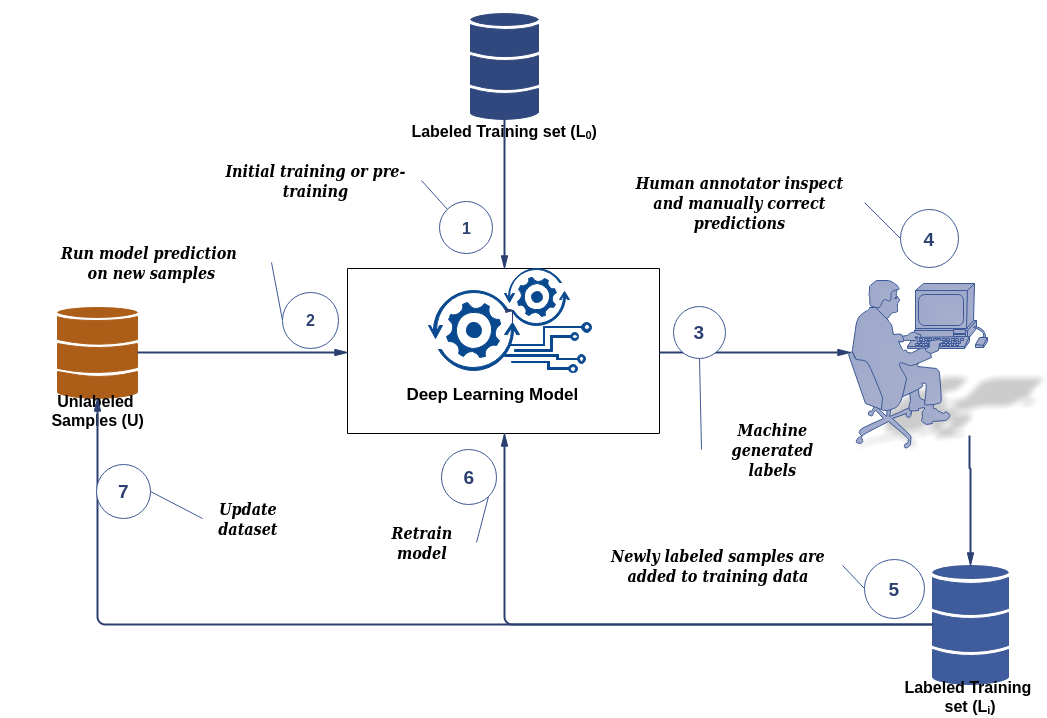
\includegraphics[width=1\linewidth]{Semi-automated IA pipeline2.png}}
			\caption{Processing pipeline of the proposed semi-automated image annotation tool. L$ _{0} $
 is the initial manually labeled dataset where L$ _{i} $
is the initial dataset plus newly labeled
samples at the $ i^{th} $ iteration.}
			\label{fig1}
		\end{figure}		
		
\section{Experimental setup and Results}
	This section of the paper explains all the necessary steps followed to prepare the environment and run the experiments. It starts by discussing how the dataset was acquired, tools and
techniques used to prepare it for training our custom Mask RCNN learning model. It covers
the type of network and configurations used, and also the steps and techniques followed
during training of the network. It concludes by presenting the results of all the experiments performed.
	
	\subsection{Raw Dataset}
	
		In this paper, we make use of XRT image dataset sourced from Machine Intelligence
Department, De Beers Technologies-South Africa. The raw data was acquired from a
diamond sorting machine which employs an X-Ray camera to capture images of crushed mineral ore particles as they are conveyed to their separation chambers. The dataset contains 3318 JPG images of 1080 * 100 (w*h) pixels, each consisting
of different object density of variable sizes, presented in fig. \ref{XRT Image}. The raw images contains leading and trailing convey belt pixels. The regions are clipped off during the pre-processing stage before data is loaded into the learner.

		\begin{figure}[htbp]
			\centering
			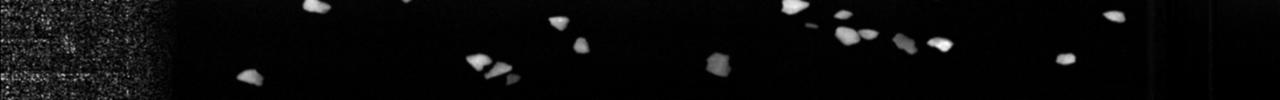
\includegraphics[width=1\linewidth]{scaled_CameraData20170505_150519_006199056_38672.jpg}
			
			\vspace{.1cm}
			
			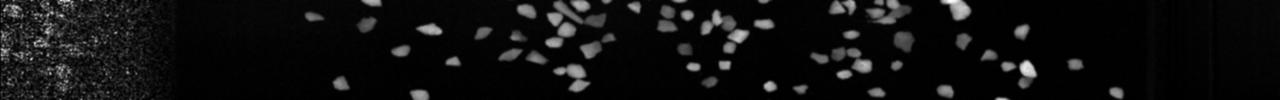
\includegraphics[width=1\linewidth]{scaled_CameraData20170505_150519_006198940_38556.jpg}
			
			\vspace{.1cm}
			
			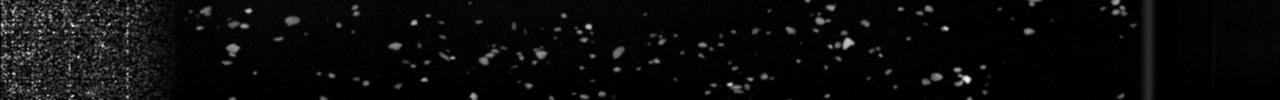
\includegraphics[width=1\linewidth]{scaled_CameraData20170505_131205_005799188_32020.jpg}
			\caption{ Raw X-ray Transmission Images}
			\label{XRT Image}
		\end{figure}
		
	\subsection{Experiment Dataset}
		
		A subset of 50 images (\textit{with a total of $\approx$ 1000 object instances of variable size}) was selected and manually labeled. The images in this subset
consists of less dense and clearly visible (\textit{less ambiguous object boundaries}) object instances, slightly dispersed with very few or none touching and / overlapping, thus easy
to manually label and less prone to annotation errors. The motive behind the selection criteria of the initial training samples was to train a model to automatically generate easy annotations and gradually incorporate more complex phenomenon like touching or
 clamping, highly dense and small objects on subsequent training iterations, guided by the human annotator. The dataset was further subdivided into 60\% (30 images) training dataset, 20\% (10 images) validation dataset and 20\% testing dataset (based on commonly
used split ratios in prior researches).\\
		
		The labeled dataset was manually annotated using VGG Image Annotator, also known as VIA \cite{Dutta}, which is a stand alone self contained web application. VIA is developed at the Visual Geometry Group (VGG) and released under the BSD-2 clause license which allows it to be useful for both academic projects and commercial applications. VIA is based entirely on HTML, javascript and css and does not require any library or additional dependencies. The system is very simple and have a minimal learning curve. The annotations can be exported to a number of different formats including: CSV and JSON, where each mask is a set of polygon points. Fig. \ref{XRT Ground-truth} depicts a manually labeled XRT image from our labeled dataset usigng VIA.
		
		\begin{figure}[htbp]
			\centering
			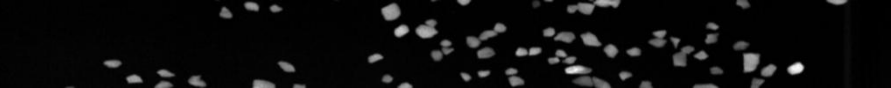
\includegraphics[width=1\linewidth]{2-raw-image.png}
			
			\vspace{.1cm}
			
			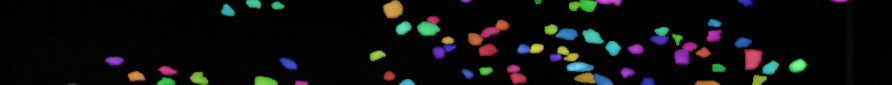
\includegraphics[width=1\linewidth]{2-ground-truth.png}
			\caption{A preview of a manually annotated XRT image.}
			\label{XRT Ground-truth}
		\end{figure}
	

	\subsection{Mask R-CNN}
		
		This research work make use of the Matterport implementation of Mask RCNN (framework
designed primarily for object instance segmentation). The implementation offers classes
that you can inherit from and provide problem specific implementation:
		
		\begin{enumerate}
			\item \textbf{Config Class}: The class consists of various hyperparameters involved during training, defined in \textbf{\textit{config.py}} file. Our custom configuration class inherit most of the default hyperparameters available with a few changes on the ones deemed to be most relevant to this research.
			
			\item \textbf{Dataset class}: A generic base class for the dataset, defined in utils.py. To add functionality specific to our custom images dataset, we inherit from this class and implement
			super class methods, \textbf{\textit{load\_mask}}, \textbf{\textit{load\_dataset}} and \textbf{\textit{load\_image}}
		\end{enumerate}
	
	\subsection{Network Training}
		
		To perform different experiments and to study the effectiveness of transfer	learning and cooperative learning, as applied to instance segmentation of XRT images, two (2) Mask R-CNN networks were trained. The first model that employs transfer learning
was initialized with MS COCO pre-trained weights and the second model was trained from scratch. Network configurations or hyperparameters were kept the same for both models.	The experiments was conducted for seven (7) training iterations. The number of epochs per
iteration was set to an arbitrary value of 50 and a regularization technique, \textbf{early stopping},
was utilized to monitor the mask validation loss (\textbf{\textit{val\_mrcnn\_mask\_loss}}) during training.
Early Stopping technique stops network training when parameter updates no longer begin
to yield an improvement on a validation set after a set of predefined epochs, referred to as
patience. We also set patience to an arbitrary value of 10, which means that we wait for 10
epochs before training is stopped if there is no performance improvement. This techniques
helps to insure that our model does not under-fit nor over-fit and fail to generalize well on
unseen image data.
\\
		
		At the end of each training cycle, 50 new images are selected from a pool of unlabeled
image dataset. The selected dataset is then subjected to automatic object detection using
the newly trained model with higher mean average precision value (mAP). The machine
generated predictions are then sent to the human annotator for inspection and manual
correction if need be, and included into the labeled dataset to form part of the ground	truth. This means that on each iteration, the previous dataset increase by 50 new more
annotated images. During selection of these images on subsequent training iteration, we
also introduced a bit more complex images: consisting of touching or overlapping, highly
dense and small particles to form part of our ground truth dataset.\\
		
	\subsection{Results}
	
		The empirical results of the two models under observation are presented in this section. We
look at the influence of transfer learning on the models as the number of training iterations
and the amount of annotated data increases.\\
		
		Table \ref{table} shows the average precision (AP) results computed over a range of 10 IoU thresholds (\textbf{\textit{from 0.5 to 0.95 with a step size of 0.05}}) for 7 training iterations. According to the results, a model that employs transfer learning recorded an
overall mAP of 55\% while a model trained from scratch recorded an mAP of 39\%. There is also a significant
overall performance difference of 16\% between the two models.
		
		
		\begin{table}[htbp]
			\caption{Object detection mAPs (\%) at different IOU threshold on XRT test images over 7 training iterations.} 
			\centering
			\begin{tabular}{|c|c|c|c|c|}
				\hline
				& \multicolumn{2}{|c|}{\textbf{Transfer Learning\newline (mAP)}}
				& \multicolumn{2}{|c|}{\textbf{No-Transfer Learning\newline (mAP)}}\\ 
				
				\hline
				Iteration & @.5 & @[0.5, 0.95] & @.5 & @[0.5, 0.95]\\
				
				\hline
				1 & 0.907 & 0.457  & 0.830 & 0.332\\
				
				\hline
				2 & 0.965 & 0.529 & 0.848 & 0.395\\
				
				\hline
				3 & 0.935 & 0.551 & 0.886 & 0.455\\
				
				\hline
				4 & 0.972 & 0.558 & 0.789 & 0.395\\
				
				\hline
				5 & 0.970 & 0.578& 0.794 & 0.395 \\
				\hline
				
				6 & 0.940 & 0.588 & 0.777 & 0.324\\
				
				\hline
				7 & 0.948 & 0.560& 0.868 & 0.429 \\
				\hline
				\textbf{Average}& & 0.546& & 0.389\\	
				\hline	
			\end{tabular} 
			\label{table}
		\end{table}

		The results in fig. \ref{mAP-cycles}, depicts average performance achieved at each training iteration for the two models. A model initialized with pretrained weights (Transfer learning model) recorded an mAP of 46\% at the beginning or initial training iteration. Its performance continues to increase
gradually as the number of training cycle and / as the domain knowledge (annotated dataset) increases . At the seventh (7$ ^{th} $) iteration, we observed a slight performance degradation of 3\% (from 59\% to 56\%). The graph of a model trained from scratch (non-Transfer Learning model) exhibits an unsteady behavior where performance of the model fluctuates across all training cycles. The model gained an linear increase in performance in the first three iteration reaching a maximum peak performance of 46\% at the 3$ ^{rd} $ iteration. We
 also observed a drastic performance degradation from the 4$ ^{th} $ to the 6$ ^{th} $ training iteration, recording the least mAP value of 32\% at the 6$ ^{th} $ iteration.
	
		\begin{figure}[htbp]
			\centering
			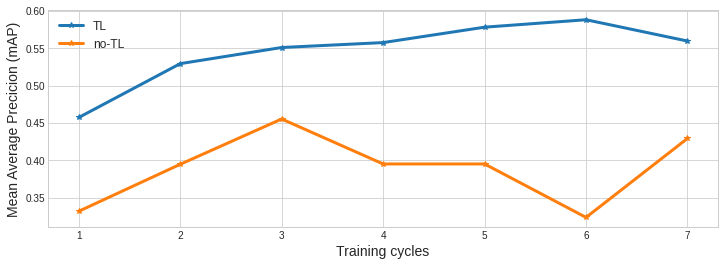
\includegraphics[width=1\linewidth]{mAP-cycles.png}
			\caption{Overall performance of our custom Mask RCNN model over 7 iterations.}
			\label{mAP-cycles}
		\end{figure}
	

\section{Discussion}
	
	In view of the results obtained, Table. \ref{table}, we recorded a high AP at the minimum IoU threshold of 0.5 and a gradual decline in AP until it reaches a value of 0 at the maximum
 IoU threshold of 0.95. This implies that more objects were detected (\textit{high true positive}) with
 atleast 50\% overlap between ground truth object mask and model predicted object mask.\\
		
	According to the results, AP values and IoU threshold values are inversely proportional. This relationship is a clear indication that the boundaries of objects detected were not accurately identified by the models. Thus an increase in percentage of overlap between (predicted, ground truth) mask pair rendered some of positive detection as negative detection. An AP of zero (0) at the maximum IoU threshold means that there is no model predicted object mask with atleast 95\% overlap with ground truth object mask. We started training our models using simple data and gradually introducing more complex data at t$ ^{he 4th} $ training iteration. We experienced a performance degradation on model
trained from scratch due to this change in the form of training samples used, which consists of touching/ overlapping and small object particles of high density with the existence of clumps. However, the model that employs transfer learning showed resilience to changes brought by this complexity in training examples. We recorded the least performance increment of 0.7\% from 55.1\% in the 3$ ^{rd} $ iteration to 55.8\% in the 4$ ^{th} $ iteration on a model that
employs transfer learning whereas its rival model recorded a declined of 6\% in performance.\\
	
	Figure \ref{mAP-cycles} shows that in the first training cycle we recorded a jump-start of 12.5\% in performance by using transfer learning. This is a significant improvement in performance particularly for a CNN model trained with small dataset of 350 labeled images. Even though we had a drop in performance at the 7th iteration we still recorded a large difference in
performance of 13.1\% between the two model. This is a clear indication that indeed transfer
learning has a considerable benefits when it comes to training of deep neural network in
cases where annotated dataset is very limited.\\
		
	With regards to cooperative sharing of annotation efforts between a human annotator and the model, we observed that our model performs poorly when it comes to small, touching/ overlapping and highly dense object particles. This still poses a lot of annotation
burdens on the human annotator as more falsely classified object boundaries had to be
corrected. Moreover, annotation of most of these particles was also very confusing and not
clear to the human eye and might have led to training of a model with false data due to
ambiguous object boundaries. This could be a possible explanation as to why we had a
drop in performance at the 7th iteration.
		
\section{Conclusion}
	
	In this research work, we proposed a semi-automated image annotation tool that incorporates machine learning and human intelligence to annotate XRT images with the ultimate
goal of establishing ground truth information. The tool provides visual feedback on machine generated annotation for the user to intercept and correct by adding missing annotations or
adjusting predicted annotation (object contours). Incorporating humans in the loop on
machine-generated annotation demonstrated significant potential benefits. The approach
effectively reduces human annotation effort and the time spent to annotate individual
images as only misclassified objects are subjected to manual annotation. In the initial
training stages, we experienced a large number of misclassified objects and gradually reduces
as more knowledge about the subject domain increases with training cycles. However,
as more complex training examples (small particle, touching, overlapping and some with
the presence of clumps) are introduced at every training cycle, we experience very slow
performance gain. Moreover, some objects’ contours or boundaries are very ambiguous
and confusing to the human eye which poses a threat of training a model with bad data or
noisy data.\\
	
	Our empirical results demonstrate that integrating prior knowledge from previous tasks
during training of CNN, (Mask-RCNN) is efficient and provides a promising results despite small ground truth information about the subject domain of the novel task. However,
training from scratch is computationally expensive and requires more training examples
to reach a comparable achievable performance to model that employs transfer learning.\\
	
	The main contribution of this paper represents an annotated XRT image dataset
and a tool that facilitate semi-automated image annotation of XRT images at pixel level
accuracy. The dataset can be used in further researches involving XRT images. By the time
of conducting this research, there was very limited prior work on instance segmentation
of XRT particles images, thus this research work also serves as a baseline for further
improvement of the XRT image detection models.\\
	
	However, this research work did not perform an exhaustive exploration of the network
hyperparameters which possibly limited the results obtained. The hyperparameters that
are worth taking into consideration in future works include, lowering the backbone model
capacity from the default ResNet-101 to shallow networks like ResNet-32 and ResNet-20. This is based on the empirical evidence from the ResNet paper\cite{Ren} which shows that
classification error on CIFAR-10 dataset decreases with increasing number of layers in
ResNet up until ResNet-1208. ResNet-1202 actually performs worse that ResNet-20 and
this could also be the case with our model since training dataset is very small and might
not need very deep network backbone. Another important factor that should be taken into
account is the correlation between images used to train the backbone network and our XRT
images and try a different network backbone trained with images that resembles or share a
lot of features in common with XRT images.
Another important aspect that was not considered in this thesis but could be incooperated
in future is the use of crowd-sourcing approach on machine generated prediction. This
involves obtaining different validation from a group of human annotators, domain experts
if possible, and fuse the annotation results. The process can help to reduce if not eliminate
ambiguity on revised machine generated annotations and avoid training with subjectively
bad data on subsequent training iterations.


\begin{thebibliography}{00}
	
	\bibitem{b1} S. L. S. Abdullah, H. Hambali, and N. Jamil, “An accurate thresholding-based segmentation technique for natural images,” SHUSER 2012 - 2012 IEEE Symposium on
Humanities, Science and Engineering Research, pp. 919–922, 2012.
	\bibitem{b2} Q. Cheng, Q. Zhang, P. Fu, C. Tu, and S. Li, “A survey and analysis on automatic
image annotation,” Pattern Recognition, vol. 79, no. June, pp. 242–259, 2018.
	\bibitem{b3} J. Jeon, V. Lavrenko, and R. Manmatha, “Automatic Image Annotation and Retrieval
using Cross-Media Relevance Models Categories and Subject Descriptors,” Proceedings
of the 26th International ACM SIGIR Conference, pp. 119–126, 2003.
	\bibitem{b4} V. Lavrenko, R. Manmatha, and J. Jeon, “A model for learning the semantics of
pictures,” Advances in Neural Information Processing Systems, 2004.
	\bibitem{b5} S. L. Feng, R. Manmatha, and V. Lavrenko, “Multiple Bernoulli relevance models for
image and video annotation,” Proceedings of the IEEE Computer Society Conference
on Computer Vision and Pattern Recognition, vol. 2, 2004.
	\bibitem{b6} A. Makadia, V. Pavlovic, and S. Kumar, “A New Baseline for Image Annotation,” pp. 1–14.
	\bibitem{b7} K. Akhilesh and R. R. Sedamkar, “Automatic image annotation using an ant colony
optimization algorithm (ACO),” 2016 IEEE 7th Power India International Conference,
PIICON 2016, pp. 1–4, 2017.
	\bibitem{meanShift} C. Peter, A, IEEE, N. O. Machine, and V. O. L. Intelligence, “Mean Shift: A Robust
Approach Toward Feature Space Analysis.,” on Pattern Analysis and 5MAY, vol. 24,
no. 5, pp. 603–619, 2002.
	\bibitem{IAGA} S. Bahrami and M. Saniee Abadeh, “Automatic Image Annotation Using an Evolutionary Algorithm (IAGA),” 2014 7th International Symposium on Telecommunications,
IST 2014, pp. 320–325, 2014.
	\bibitem{MLMC} H. Wang and J. Hu, “Multi-label image annotation via maximum consistency,” Proceedings - International Conference on Image Processing, ICIP, pp. 2337–2340, 2010.
	\bibitem{Wang} H. Wang, H. Huang, and C. Ding, “Image annotation using multi-label correlated
Green’s function,” Proceedings of the IEEE International Conference on Computer
Vision, no. Iccv, pp. 2029–2034, 2009.
	\bibitem{LSR} Z. Lin, G. Ding, M. Hu, J. Wang, and X. Ye, “Image tag completion via image-specific
and tag-specific linear sparse reconstructions,” Proceedings of the IEEE Computer
Society Conference on Computer Vision and Pattern Recognition, pp. 1618–1625, 2013.
	\bibitem{TCFIR} L. Wu, R. Jin, and A. K. Jain, “Tag completion for image retrieval,” IEEE Transactions on Pattern Analysis and Machine Intelligence, vol. 35, no. 3, pp. 716–727, 2013.
	\bibitem{ITCR} Y. Hou and Z. Lin, “Image tag completion and refinement by subspace clustering and
 matrix completion,” 2015 Visual Communications and Image Processing, VCIP 2015,
no. Imc, pp. 1–4, 2016
	\bibitem{Simonyan} K. Simonyan, A. Vedaldi, and A. Zisserman, “Deep Inside Convolutional Networks: Visualising Image Classification Models and Saliency Maps,” pp. 1–8, 2013.
	\bibitem{Shin} H. C. Shin, H. R. Roth, M. Gao, L. Lu, Z. Xu, I. Nogues, J. Yao, D. Mollura, and R. M. Summers, “Deep Convolutional Neural Networks for Computer-Aided Detection: CNN Architectures, Dataset Characteristics and Transfer Learning,” IEEE Transactions on Medical Imaging, vol. 35, no. 5, pp. 1285–1298, 2016.
	\bibitem{Kalita} S. Kalita and M. Biswas, “Improved Convolutional Neural Networks for Hyperspectral Image Classification,” Advances in Intelligent Systems and Computing, vol. 740, pp. 397– 410, 2019.
	\bibitem{Zhu} S. Shen, S. Zhu, Z. Shi, and C. Sun, “Deep neural network based image annotation,” Pattern Recognition Letters, vol. 65, pp. 103–108, 2015.
	\bibitem{kivinen} J. Kivinen and M. K. Warmuth, “Exponentiated Gradient versus Gradient Descent for	Linear Predictors,” Information and Computation, vol. 132, no. 1, pp. 1–63, 1997.
	\bibitem{Gong} Y. Gong, Y. Jia, T. Leung, A. Toshev, and S. Ioffe, “Deep Convolutional Ranking for
Multilabel Image Annotation,” pp. 1–9, 2013.
	\bibitem{Hinton} E. Hinton, “ImageNet Classicafication with Deep Convolutional Networks,” Handbook of Approximation Algorithms and Metaheuristics, pp. 60–1–60–16, 2007.
	\bibitem{Cao} J. Cao, C. Wu, L. Chen, H. Cui, and G. Feng, “An Improved Convolutional Neural
Network Algorithm and Its Application in Multilabel Image Labeling,” Computational
Intelligence and Neuroscience, vol. 2019, pp. 1–12, 2019.
	\bibitem{Mayhew} M. B. Mayhew, B. Chen, and K. S. Ni, “Assessing semantic information in convolutional neural network representations of images via image annotation,” Proceedings -
International Conference on Image Processing, ICIP, vol. 2016-Augus, pp. 2266–2270,
2016.
	\bibitem{Kai} H. Kai, “Deep Multiple Instance Learning for Image Classification and
 Auto-Annotation,” Journal of Reconstructive Microsurgery, vol. 1, no. 4, pp. 287–289,
2013
	\bibitem{Dutta} A. Dutta, A. Gupta, and A. Zissermann, “VGG image annotator (VIA).”
 http://www.robots.ox.ac.uk/ vgg/software/via/, 2016. Version: X.Y.Z, Accessed:02/03/2020
	\bibitem{Ren} K. He, X. Zhang, S. Ren, and J. Sun, “Deep residual learning for image recognition,”
Proceedings of the IEEE Computer Society Conference on Computer Vision and Pattern
Recognition, vol. 2016-December, pp. 770–778, 2016.
 
\end{thebibliography}
\vspace{12pt}
\end{document}
